% Random city
% Author: Pascal Seppecher
\documentclass[tikz,border=10pt]{standalone}
%%%<
\usepackage{verbatim}
%%%>
\begin{comment}
:Title: Random city
:Tags: Background;Coordinate calculations;Scopes;3D;Random;Architecture
:Author: Pascal Seppecher
:Slug: city

An isometric view of a random city.
\end{comment}
\usetikzlibrary{backgrounds}
\usepackage{ifthen}
% The blue print color
\definecolor{blueprintcolor}{RGB}{20,20,100}

% The shadow color
\colorlet{shadow}{blueprintcolor!50!white}

% The light color
\colorlet{light}{white!90!blueprintcolor}


\tikzset{every picture/.style={line width=0.75pt}} %set default line width to 0.75pt        


\begin{document}
% Draws a hundred blocks random city




\tikzset{every picture/.style={line width=0.75pt}} %set default line width to 0.75pt        



\tikzset{every picture/.style={line width=0.75pt}} %set default line width to 0.75pt        

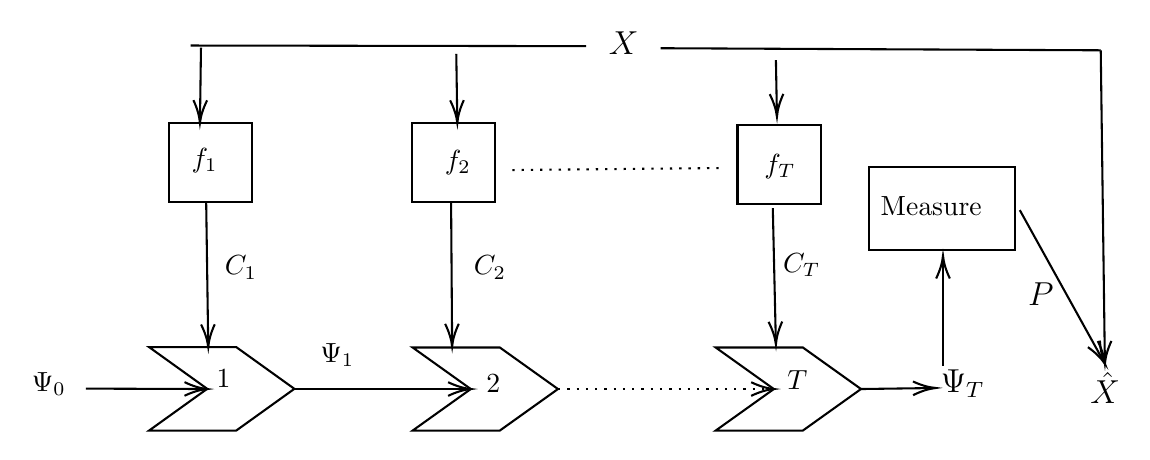
\begin{tikzpicture}[x=0.75pt,y=0.75pt,yscale=-1,xscale=1]
%uncomment if require: \path (0,300); %set diagram left start at 0, and has height of 300

%Chevron Arrow [id:dp3838926820938916] 
\draw   (88,166.8) -- (130,166.8) -- (158,186.9) -- (130,207) -- (88,207) -- (116,186.9) -- cycle ;
%Chevron Arrow [id:dp7442417894924472] 
\draw   (361,167) -- (403,167) -- (431,187) -- (403,207) -- (361,207) -- (389,187) -- cycle ;
%Chevron Arrow [id:dp8109207930156583] 
\draw   (215,167) -- (257,167) -- (285,187) -- (257,207) -- (215,207) -- (243,187) -- cycle ;
%Straight Lines [id:da8862657240629535] 
\draw    (57.5,186.8) -- (114,186.99) ;
\draw [shift={(116,187)}, rotate = 180.2] [color={rgb, 255:red, 0; green, 0; blue, 0 }  ][line width=0.75]    (10.93,-3.29) .. controls (6.95,-1.4) and (3.31,-0.3) .. (0,0) .. controls (3.31,0.3) and (6.95,1.4) .. (10.93,3.29)   ;
%Straight Lines [id:da7975298110809533] 
\draw    (158,187) -- (241,187) ;
\draw [shift={(243,187)}, rotate = 180] [color={rgb, 255:red, 0; green, 0; blue, 0 }  ][line width=0.75]    (10.93,-3.29) .. controls (6.95,-1.4) and (3.31,-0.3) .. (0,0) .. controls (3.31,0.3) and (6.95,1.4) .. (10.93,3.29)   ;
%Straight Lines [id:da6215403158330051] 
\draw  [dash pattern={on 0.84pt off 2.51pt}]  (285,187) -- (387,187) ;
\draw [shift={(389,187)}, rotate = 180] [color={rgb, 255:red, 0; green, 0; blue, 0 }  ][line width=0.75]    (10.93,-3.29) .. controls (6.95,-1.4) and (3.31,-0.3) .. (0,0) .. controls (3.31,0.3) and (6.95,1.4) .. (10.93,3.29)   ;
%Straight Lines [id:da83415619681525] 
\draw    (431,187) -- (465,186.53) ;
\draw [shift={(467,186.5)}, rotate = 539.2] [color={rgb, 255:red, 0; green, 0; blue, 0 }  ][line width=0.75]    (10.93,-3.29) .. controls (6.95,-1.4) and (3.31,-0.3) .. (0,0) .. controls (3.31,0.3) and (6.95,1.4) .. (10.93,3.29)   ;
%Straight Lines [id:da6413960895162699] 
\draw    (470.5,175.8) -- (470.5,124.8) ;
\draw [shift={(470.5,122.8)}, rotate = 450] [color={rgb, 255:red, 0; green, 0; blue, 0 }  ][line width=0.75]    (10.93,-3.29) .. controls (6.95,-1.4) and (3.31,-0.3) .. (0,0) .. controls (3.31,0.3) and (6.95,1.4) .. (10.93,3.29)   ;
%Shape: Rectangle [id:dp7601935244032024] 
\draw   (435,80) -- (505,80) -- (505,120) -- (435,120) -- cycle ;
%Shape: Rectangle [id:dp8110460816862144] 
\draw   (97.5,59) -- (137.5,59) -- (137.5,96.8) -- (97.5,96.8) -- cycle ;
%Shape: Rectangle [id:dp7599425283365432] 
\draw   (214.5,59) -- (254.5,59) -- (254.5,96.8) -- (214.5,96.8) -- cycle ;
%Shape: Rectangle [id:dp53670336511919] 
\draw   (371.5,60) -- (411.5,60) -- (411.5,97.8) -- (371.5,97.8) -- cycle ;
%Straight Lines [id:da6858267831505039] 
\draw    (113,22.5) -- (112.53,56.8) ;
\draw [shift={(112.5,58.8)}, rotate = 270.79] [color={rgb, 255:red, 0; green, 0; blue, 0 }  ][line width=0.75]    (10.93,-3.29) .. controls (6.95,-1.4) and (3.31,-0.3) .. (0,0) .. controls (3.31,0.3) and (6.95,1.4) .. (10.93,3.29)   ;
%Straight Lines [id:da05714674442064638] 
\draw    (236,25.5) -- (236.47,56.8) ;
\draw [shift={(236.5,58.8)}, rotate = 269.14] [color={rgb, 255:red, 0; green, 0; blue, 0 }  ][line width=0.75]    (10.93,-3.29) .. controls (6.95,-1.4) and (3.31,-0.3) .. (0,0) .. controls (3.31,0.3) and (6.95,1.4) .. (10.93,3.29)   ;
%Straight Lines [id:da17304639439275682] 
\draw    (108,21.5) -- (298.5,21.8) ;
%Straight Lines [id:da22853807737691667] 
\draw    (334.5,22.8) -- (546.5,23.8) ;
%Straight Lines [id:da7792326099304743] 
\draw    (390,28.5) -- (390.46,53.8) ;
\draw [shift={(390.5,55.8)}, rotate = 268.95] [color={rgb, 255:red, 0; green, 0; blue, 0 }  ][line width=0.75]    (10.93,-3.29) .. controls (6.95,-1.4) and (3.31,-0.3) .. (0,0) .. controls (3.31,0.3) and (6.95,1.4) .. (10.93,3.29)   ;
%Straight Lines [id:da8122774513040364] 
\draw    (507.5,100.8) -- (547.53,173.05) ;
\draw [shift={(548.5,174.8)}, rotate = 241.01] [color={rgb, 255:red, 0; green, 0; blue, 0 }  ][line width=0.75]    (10.93,-3.29) .. controls (6.95,-1.4) and (3.31,-0.3) .. (0,0) .. controls (3.31,0.3) and (6.95,1.4) .. (10.93,3.29)   ;
%Straight Lines [id:da5170940357988966] 
\draw    (546.5,23.8) -- (548.47,172.8) ;
\draw [shift={(548.5,174.8)}, rotate = 269.24] [color={rgb, 255:red, 0; green, 0; blue, 0 }  ][line width=0.75]    (10.93,-3.29) .. controls (6.95,-1.4) and (3.31,-0.3) .. (0,0) .. controls (3.31,0.3) and (6.95,1.4) .. (10.93,3.29)   ;
%Straight Lines [id:da14382493284374753] 
\draw    (115.5,96.8) -- (116.47,164.8) ;
\draw [shift={(116.5,166.8)}, rotate = 269.18] [color={rgb, 255:red, 0; green, 0; blue, 0 }  ][line width=0.75]    (10.93,-3.29) .. controls (6.95,-1.4) and (3.31,-0.3) .. (0,0) .. controls (3.31,0.3) and (6.95,1.4) .. (10.93,3.29)   ;
%Straight Lines [id:da20101360743532437] 
\draw    (388.5,99.8) -- (389.95,163.5) ;
\draw [shift={(390,165.5)}, rotate = 268.69] [color={rgb, 255:red, 0; green, 0; blue, 0 }  ][line width=0.75]    (10.93,-3.29) .. controls (6.95,-1.4) and (3.31,-0.3) .. (0,0) .. controls (3.31,0.3) and (6.95,1.4) .. (10.93,3.29)   ;
%Straight Lines [id:da08374413714558848] 
\draw    (233.5,96.8) -- (233.99,164.5) ;
\draw [shift={(234,166.5)}, rotate = 269.59000000000003] [color={rgb, 255:red, 0; green, 0; blue, 0 }  ][line width=0.75]    (10.93,-3.29) .. controls (6.95,-1.4) and (3.31,-0.3) .. (0,0) .. controls (3.31,0.3) and (6.95,1.4) .. (10.93,3.29)   ;
%Straight Lines [id:da8670780588257153] 
\draw  [dash pattern={on 0.84pt off 2.51pt}]  (263,81.5) -- (365,80.5) ;

% Text Node
\draw (119,176.4) node [anchor=north west][inner sep=0.75pt]    {$1$};
% Text Node
\draw (249,178.4) node [anchor=north west][inner sep=0.75pt]    {$2$};
% Text Node
\draw (394,176.4) node [anchor=north west][inner sep=0.75pt]    {$T$};
% Text Node
\draw (30,177.4) node [anchor=north west][inner sep=0.75pt]    {$\Psi _{0}$};
% Text Node
\draw (169,163.4) node [anchor=north west][inner sep=0.75pt]    {$\Psi _{1}$};
% Text Node
\draw (468,176.4) node [anchor=north west][inner sep=0.75pt]  [font=\large]  {$\Psi _{T}$};
% Text Node
\draw (439,93) node [anchor=north west][inner sep=0.75pt]   [align=left] {Measure};
% Text Node
\draw (510,134.4) node [anchor=north west][inner sep=0.75pt]  [font=\large]  {$P$};
% Text Node
\draw (308,13.4) node [anchor=north west][inner sep=0.75pt]  [font=\large]  {$X$};
% Text Node
\draw (107,69.4) node [anchor=north west][inner sep=0.75pt]    {$f_{1}$};
% Text Node
\draw (229,70.4) node [anchor=north west][inner sep=0.75pt]    {$f_{2}$};
% Text Node
\draw (383,72.4) node [anchor=north west][inner sep=0.75pt]    {$f_{T}$};
% Text Node
\draw (540,177.4) node [anchor=north west][inner sep=0.75pt]  [font=\large]  {$\hat{X}$};
% Text Node
\draw (123,121.4) node [anchor=north west][inner sep=0.75pt]    {$C_{1}$};
% Text Node
\draw (243,121.4) node [anchor=north west][inner sep=0.75pt]    {$C_{2}$};
% Text Node
\draw (392,120.4) node [anchor=north west][inner sep=0.75pt]    {$C_{T}$};


\end{tikzpicture}

\end{document}

